\documentclass[12pt, letterpaper]{article}
\usepackage{graphicx} % Required for inserting images
\graphicspath{{images/}} %configuring the graphicx package
\usepackage[T1]{fontenc}
\usepackage{hyperref}
\usepackage[section]{placeins}

\title{Raport zaliczeniowy}
\author{Mateusz Luberda }
\date{Czerwiec 5, 2023}

\begin{document}

\maketitle
\renewcommand*\contentsname{Spis treści}
\begingroup
  \flushbottom
  \tableofcontents
  \newpage
\endgroup

\section{Opis problemu}

Celem zadania jest zbadanie zależności słuchalności różnych artystów od czynników takich jak: wiek, kraj urodzenia, główny gatunek muzyczny, liczba różnych gatunków muzycznych grana przez muzyka, lata aktywności oraz płeć. Słuchalność danego artysty może być różnie interpretowana, dlatego na potrzeby tego badania jest ona odwrotnie proporcjonalna z miejscem na liście Billboard. Głównym problemem badawczym jest wyłonienie cech idealnych, czyli takich, które teoretycznie zagwarantują miejsce numer jeden na liście. Oczywiście na taki suckes składa się o wiele więcej czynników, często niemierzalnych, dlatego proszę potraktować wyłonienie idealnych cech jako zbadanie opini publicznej, a nie jako wyznacznik sukcesu. Dane będą pozyskiwane samodzielnie. Listy artystów pobierane są ze strony \url{https://www.billboard.com/charts/year-end/top-artists/}, a informacje o nich z wikipedii. W celu uruchomienia programu, proszę zainstalować następujące biblioteki:
\begin{itemize}
  \item billboard
  \item pandas
  \item pandas\_profiling
  \item wikipedia
  \item beautifulsoup4
  \item gender-guesser
  \item requests
  \item pandas
  \item sklearn
  \item matplotlib
\end{itemize}

\section{Pozyskiwanie danych}

\subsection{Scrapowanie}

\subsubsection{Billboard}

W celu pobrania danych ze strony \url{https://www.billboard.com/charts/year-end/top-artists/} używam biblioteki billboard. Wyróżniłem trzy funkcje:
\begin{enumerate}
    \item get\_top\_artists\_from\_year(year) - zwraca listę artystów wraz z ich miejscem w rankingu po podaniu roku utworzenia rankingu.
    \item def get\_top\_artists\_from\_year\_range(start\_year, end\_year) - zwraca listę artystów wraz z ich miejscem w rankingu po podaniu zakresu z jakiego chcemy pobrać dane. Używa get\_top\_artists\_from\_year(year)
    \item filter\_artists(start\_year, end\_year) - zwraca listę artystów w rankingu po podaniu zakresu z jakiego chcemy pobrać dane bez powtarzających się nazw. Używa get\_top\_artists\_from\_year\_range(start\_year, end\_year)
\end{enumerate}

\subsubsection{Wikipedia}

W celu pobrania informacji na temat artystów z wikipedii użyłem bibliotek wikipedia i bs4. Wyróżniłem funkcje:
\begin{enumerate}
    \item prepare\_url(artist\_name) - zwraca adres url strony wikipedii na podstawie nazwy arysty podanego w argumencie. Większość adresów na wikipedii ma postać en.wikipedia.org/wiki/artist\_name, jednak u niektórych dopisany jest komentarz w nawiasie, np. \_(band) dla zespołów, czy \_(producer) dla producentów. Jest to zamknięty zbiór takich komentarzy, więc są one zgromadzone w zmiennej globalnej i po kolei przeszukiwane dopóki nie znajdziemy strony.
    \item prepare\_infobox(url) - na podstawie adresu url strony wikipedii zwraca słownik z potrzebnymi do przetworzenia informacjami. Wyłania je, tworząc infobox, czyli szablon z podstawowymi informacjami o danym temacie. Uzywając bs4.BeatufiulSoup oraz parsera html wyróżniliśmy tylko te dane, których będziemy później używacć.
    \item extract\_info(infobox) - na podstawie przefiltrowanego infoboxa zwraca słownik z przetworzonymi danymi. Są to jeszcze dane wymagające pre-processingu Używa poniższych funkcji:
    \begin{enumerate}
        \item get\_age(infobox) - oblicza wiek artysty na podstawie daty urodzenia
        \item get\_country(infobox) - znajduje kraj pochodzenia danego artysty
        \item get\_genres(infobox) - tworzy listę gatunków muzcznych jakimi zajmuje się artysta oraz zwraca ich ilość
        \item get\_years\_active(infobox) - oblicza jak długo artysta jest aktywny w świecie muzycznym
        \item get\_gender(infobox) - zgaduje płeć artysty na podstawie jego oryginalnego imienia
    \end{enumerate}
\end{enumerate}

\subsection{Pre-processing}

Uzupełnianie i poprawa danych w tym przypadku polega na ich ujednoliceniu, ponieważ często te same dane zapisane są innymi słowami. Jeśli danych nie da się poprawić lub nie da się ich znaleźć, usuwamy je. Wyróźniłem funkcje:
\begin{enumerate}
    \item preprocessing\_age\_bands(infobox) - oblicza średni wiek w zespole muzycznym. Jeśli nie ma informacji na temat niektórych członków zespołu, zakłada, że mają oni zbliżony wiek do tych, których wiek znamy. Jeśli nie ma informacji na temat żadnego członka zespołu, zwraca None.
    \item preprocessing\_country(country) - zwraca ujednoliconą nazwę pańśtwa, tzn. usuwa niepotrzebne przecinki, nawiasy, liczby przy nazwie wcześniej pobranej. Sprawdza, czy państwo jest napisane skrótem, czy nie i sprowadza nazwę do jednej postaci.
    \item preprocessing\_genres(genres) - wybiera z listy najbardziej popularny gatunek muzyczny. Lista najbardziej popularnych gatunków jest zbiorem skończonym i zdefioniowanym jako globalna zmienna.
    \item preprocessing\_gender(sex) - dla wartości różnych od None ujednolica odpowiedź do "male" albo "female"
    \item preprocessing\_gender\_bands(infobox) - dla zespołów wybiera płeć zespołu, czyli taką jaką ma większość członków zespołu
    \item preprocessing\_dict(dict) - na podstawie słownika z danymi o artystach zwraca słownik z przetworzonymi danymi. Używa powyższych funkcji.
    \item erase\_leftovers(dict) - usuwa ze słownika z danymi o artystach wszystkie wiersze, w których wystąpiła wartość None i zwraca nowy słownik.
\end{enumerate}

\subsection{Wstępna analiza danych}
Wstępną analizę danych wygenerowano z biblioteki pandas-profiling.
Po zgromadzeniu danych i pre-processingu otrzymaliśmy tabelę z 420. artystami. Dla każdego z nich obliczyliśmy najwyższe miejsce w rankingu, wiek, określiliśmy kraj pochodzenia, najpopularniejszy gatunek muzyczny grany przez wykonawcę, liczbę róznych gatunków muzycznych jakimi posługuje się artysta, obliczyliśmy lata aktywności na scenie i zapisaliśmy płeć. Nasze ostateczne dane zgromadzone są w postaci pliku artists.csv:                                                                                                                                                                                                                                                                                                                                                                                                       
\begin{figure}[h]
    \centering
    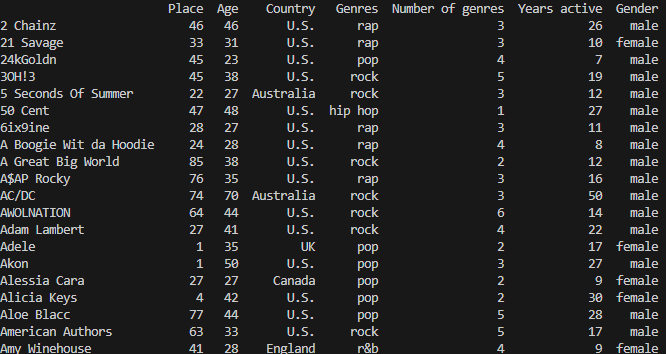
\includegraphics[width=1\textwidth]{data_head}  
    \caption{Pierwsze pięc wierszy pliku artists.csv z danymi}
\end{figure}

Macierz korelacji pokazuje nam zależność zmiennych od siebie nawzajem. Lata aktywności oraz wiek są od siebie wzajemnie mocno zależne, co jest dość oczywiste, gdyż większość artystów zaczyna swoją karierę w wieku około 20 lat. Także niezaskakującą zależnością jest państwo od gatunków i na odwrót. Każdy kraj ma dominujący gatunek muzyczny.

\begin{figure}[h]
    \centering
    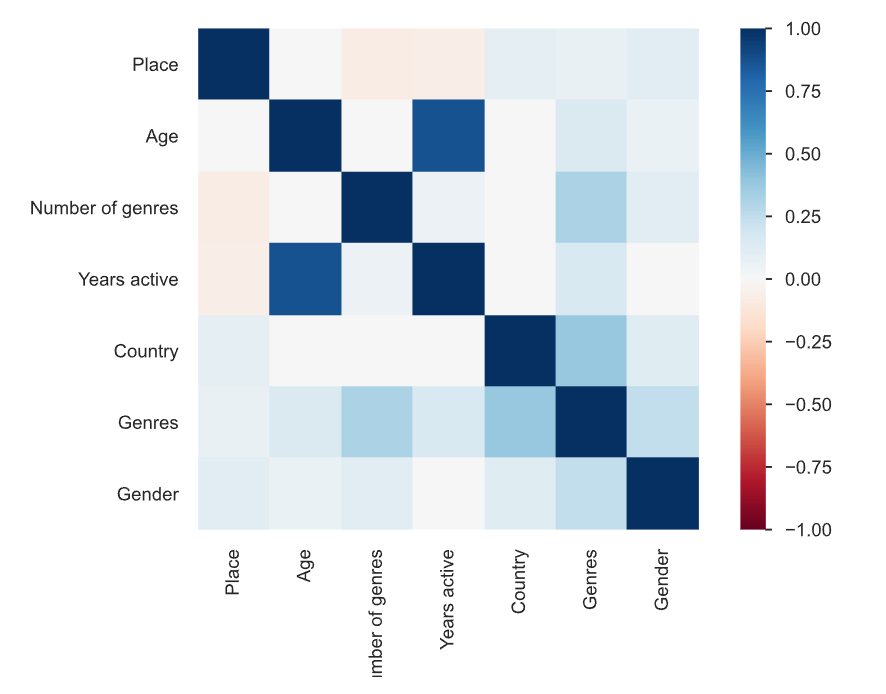
\includegraphics[width=0.8\textwidth]{correlation_matrix}  
    \caption{Macierz korelacji}
\end{figure}

\subsubsection{Wiek}

Najczęściej występującymi artystami w rankingu są wykonwacy w wieku 30-34, jednak tych oscylujących około 40. także nie brakuje. Gdy spojrzymy na zależność miejsca w rankingu od wieku widać, że dane są bardzo porozrzucane. Łatwo jednak zauważyć, że najczęściej pierwsze miejsce w rankingu mają artysci w przedziale 28-50

\begin{figure}[h]
    \centering
    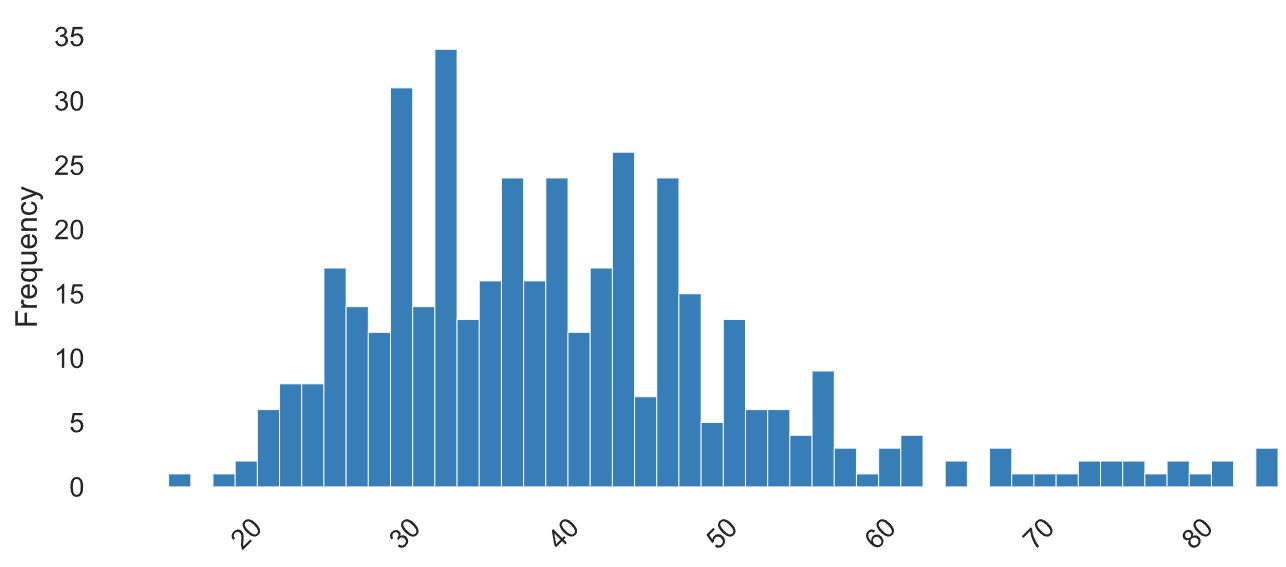
\includegraphics[width=0.5\textwidth]{age_frequency}  
    \caption{Częstotliwość wieku}
\end{figure}

\begin{figure}[h!]
    \centering
    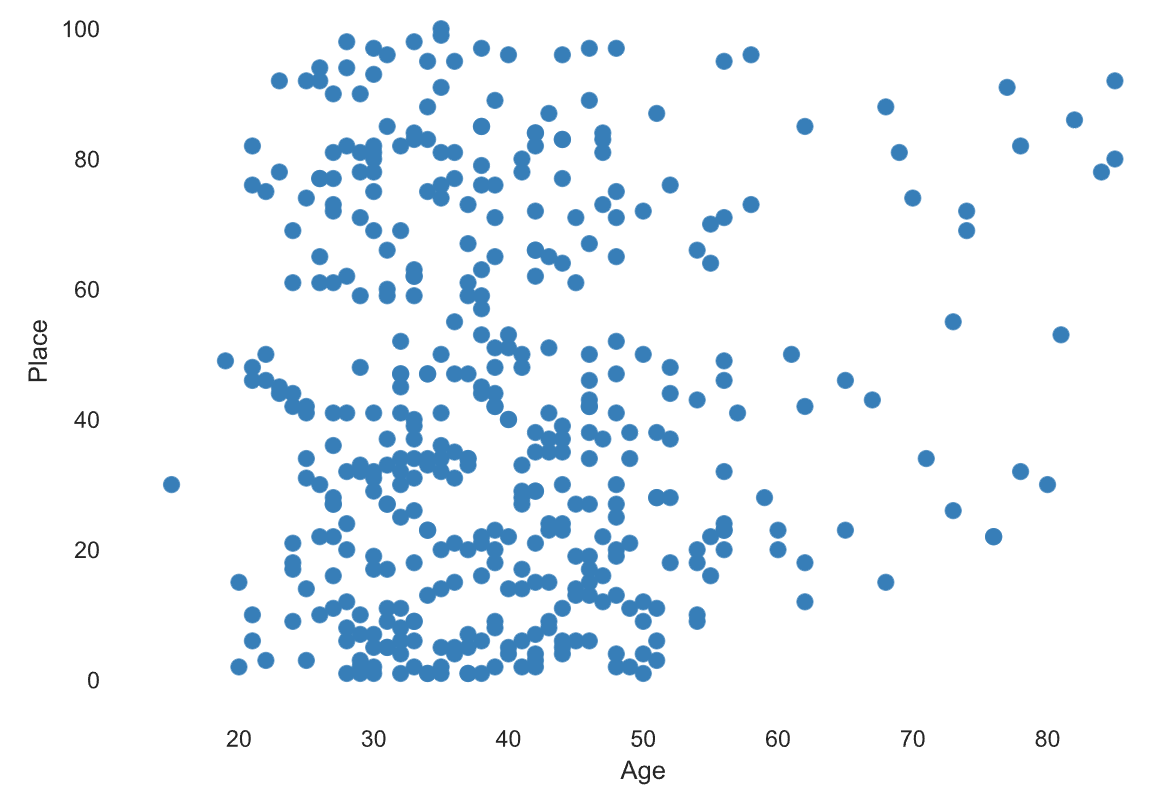
\includegraphics[width=0.5\textwidth]{place_age}  
    \caption{Zależność miejsca w rankingu od wieku}
\end{figure}

\subsubsection{Państwo}

Najczęściej występującymi artystami w rankingu są wykonwacy anglojęzyczny, którzy 4 piersze miejsca, jeżeli chodzi o częstotliwość.

\begin{figure}[h]
    \centering
    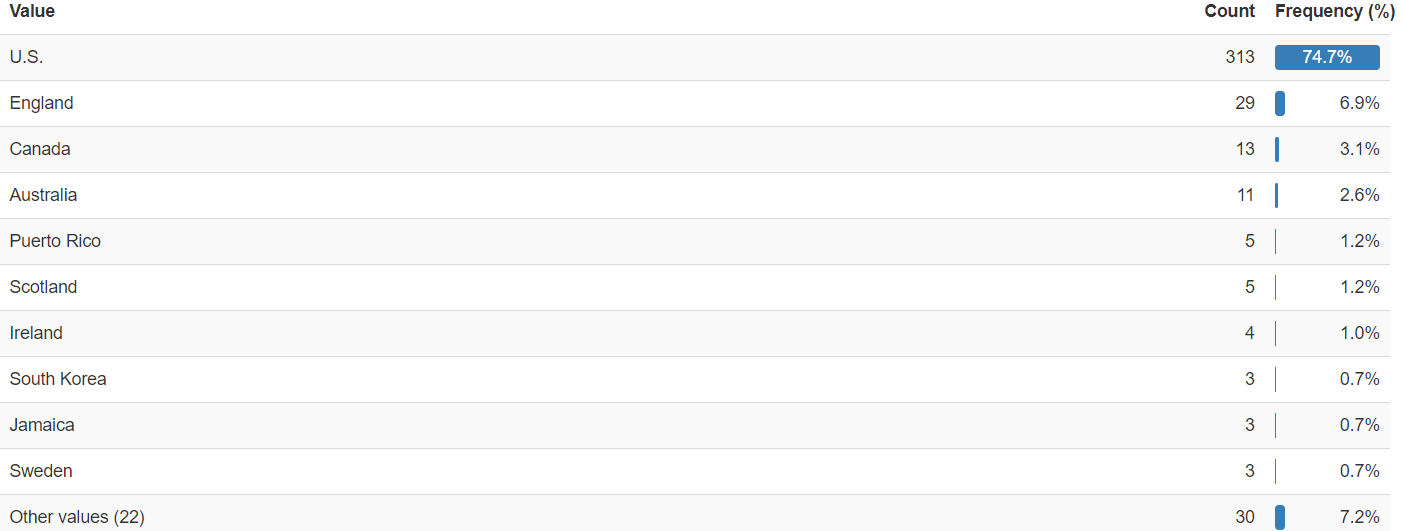
\includegraphics[width=0.8\textwidth]{country_frequency}  
    \caption{Częstotliwość państw}
\end{figure}

\subsubsection{Gatunki muzyczne}

Najczęściej występującymi arystami w rankingu są wykonwawcy rockowi lub popowi. Jeśli chodzi o różnorodnośc artysty, to zdecydowanie widać, że najczęściej w rankingu pojawiają się wykonwacy grający muzykę łączącą 3 gatunku. Na wykresie zależności miejsca w rankingu od różnorodności łatwo zauważyć, że tacy artyści też częściej mają pierwsze miejsce na liście.

\begin{figure}[h]
    \centering
    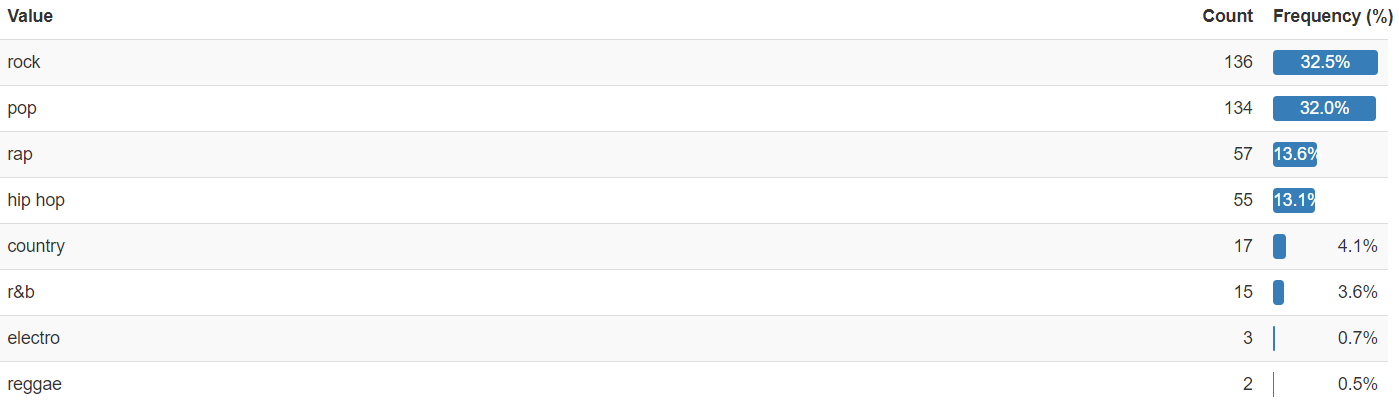
\includegraphics[width=1\textwidth]{genres_frequency}  
    \caption{Częstotliwość gatunków muzycznych}
\end{figure}

\begin{figure}[h]
    \centering
    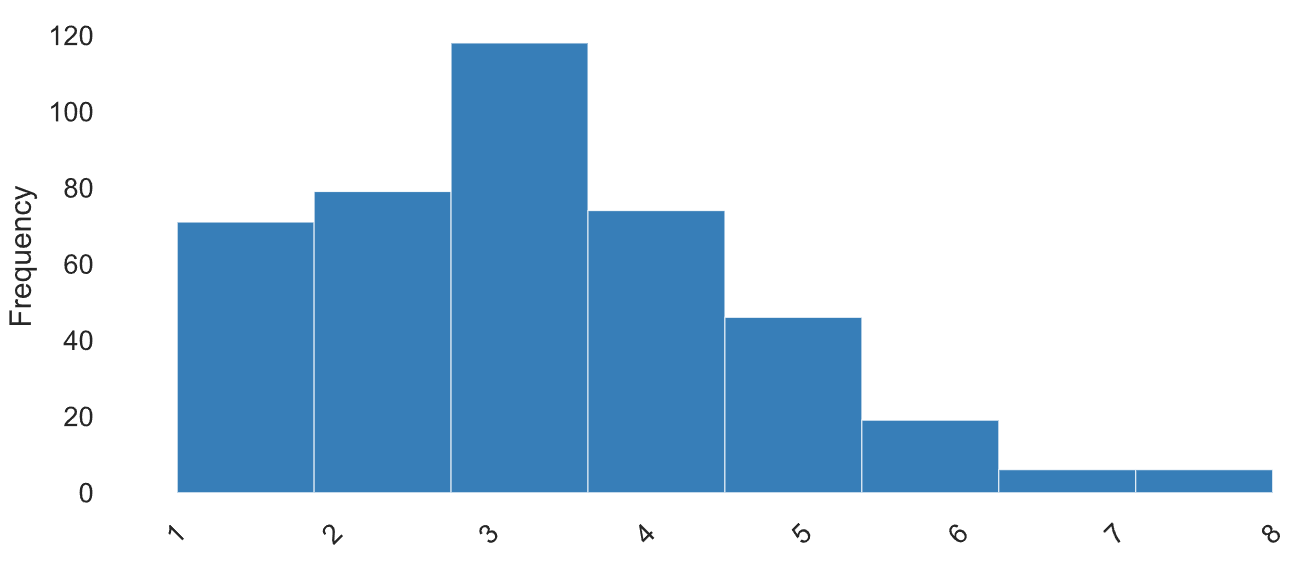
\includegraphics[width=1\textwidth]{number_of_genres_frequency}  
    \caption{Częstotliwość ilości gatunków muzycznych}
\end{figure}

\subsubsection{Lata aktywności}

Lata aktywności są ściśle powiązane z wiekiem, wiec wykresy będą przybliżone do tych wcześniej.

\begin{figure}[h]
    \centering
    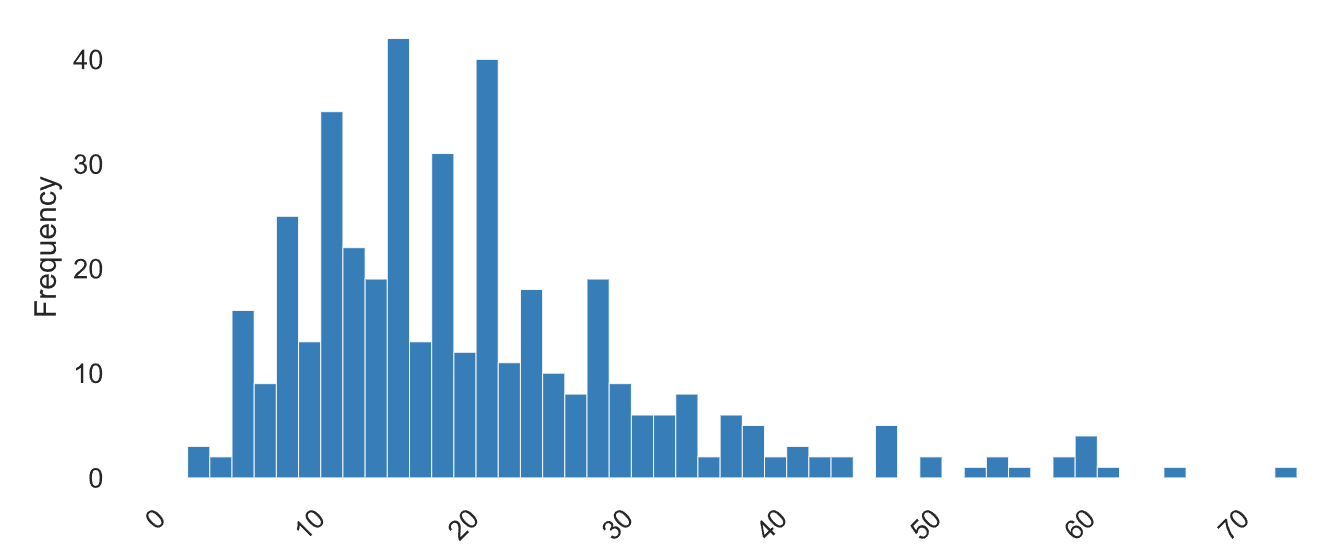
\includegraphics[width=1\textwidth]{years_active_frequency}  
    \caption{Częstotliwość lat aktywności}
\end{figure}

\begin{figure}[h]
    \centering
    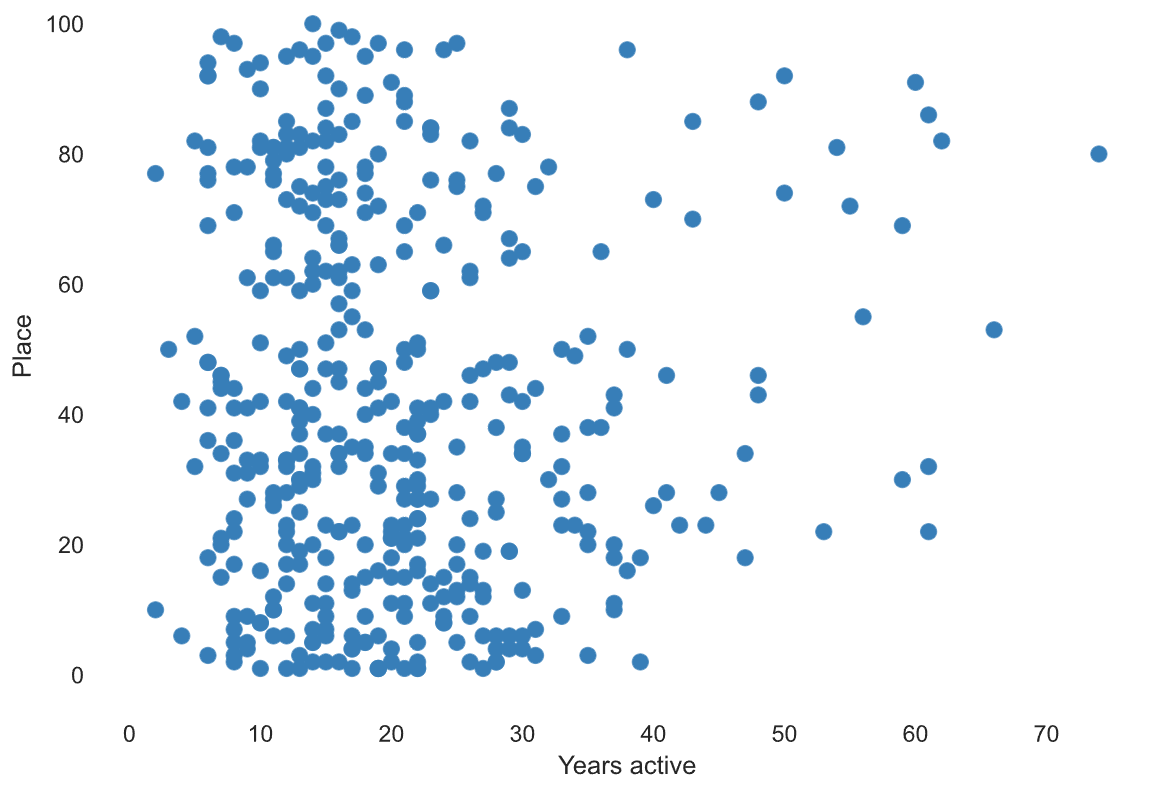
\includegraphics[width=1\textwidth]{place_years_active}  
    \caption{Zależnośc miejsca w rankingu od lat aktywności}
\end{figure}

\subsubsection{Płeć}

Rynek muzyczny zdominowali mężczyźni.

\begin{figure}[h]
    \centering
    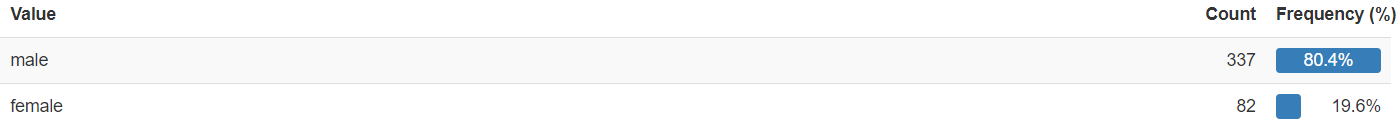
\includegraphics[width=1\textwidth]{gender_frequency}  
    \caption{Częstotliwość płci}
\end{figure}

\section{Przewidywania}

\subsection{Znaczenie zmiennych}

Zacznijmy od przebadania, która cecha najbardziej wpływa na wynik. W badaniu wpływu zmiennych na miejsce w rankingu użyłem modelu DecisionTreeClassifier, ponieważ mamy sześć zmiennych i chcemy zbadać, która z nich ma największy wpływ na wynik. Najwieksze znaczenie mają wiek oraz lata aktywności. Potem różnorodność artysty. Najmniejszy wpływ na miejsce w rankingu mają kraj, gatunki muzyczne oraz płeć. Gdy weźmiemy model, w którym rozdzielilismy zmienne na cechy kategoryczne otrzymamy bardziej szczegółowe dane. Z pańśtw pochodzenia najbardziej znaczące są USA oraz Anglia. Jesłi chodzi o gatunki muzczyne, to znowu mamy do czynienia z popem oraz rockiem. Płeć wydaje się dość zaskakująca, ponieważ mimo znacznej przewagi w ilości mężcznycn w rankingach, to artystki częściej sięgają po wyższe miejsca.

\begin{figure}[h]
    \centering
    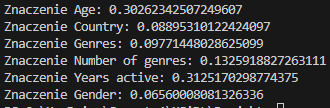
\includegraphics[width=1\textwidth]{importances}  
    \caption{Znaczenie zmiennych}
\end{figure}

\begin{figure}[h]
    \centering
    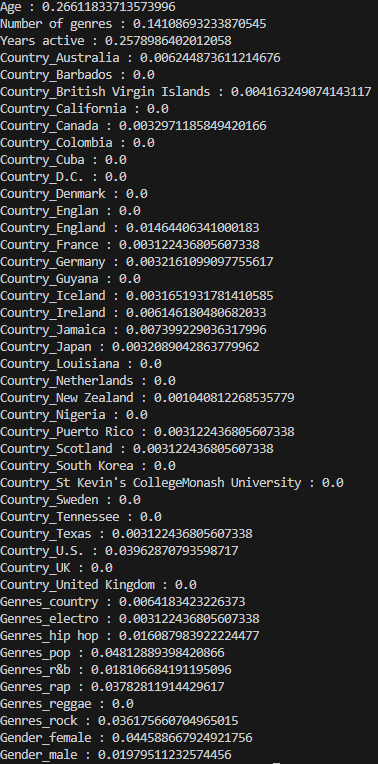
\includegraphics[width=0.65\textwidth]{importances_details}  
    \caption{Znaczenie zmiennych kategorycznych}
\end{figure}

\subsection{Wykresy przybliżające wynik}

Tworząc przybliżenia użyłem biblioteki sklearn. Biorąc pod uwagę ilość i różnorodność danych, zdeycodwałem się na wielomian 10-ego stopnia, gdyż wszystkie poniżej niewystarczająco przybliżały wyniki. Użyłem modelu LinearRegression oraz w celu podziału cech kategorycznych LabelEncoder.
\begin{figure}[h]
    \centering
    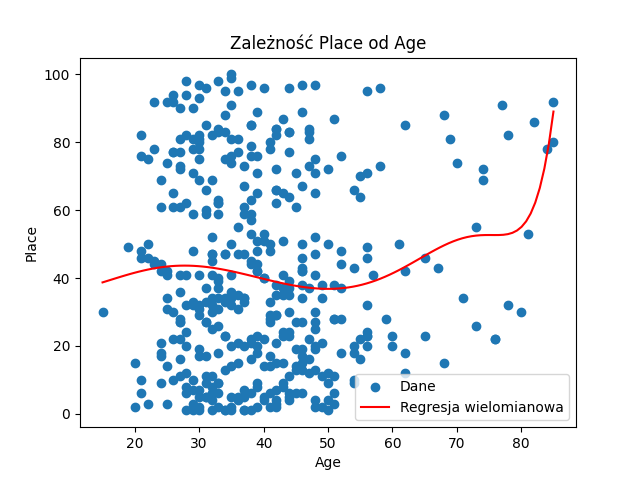
\includegraphics[width=1\textwidth]{place_age_graph}  
    \caption{Przybliżenie wielomianem zależności miejsca w rankingu od wieku}
\end{figure}

\begin{figure}[h]
    \centering
    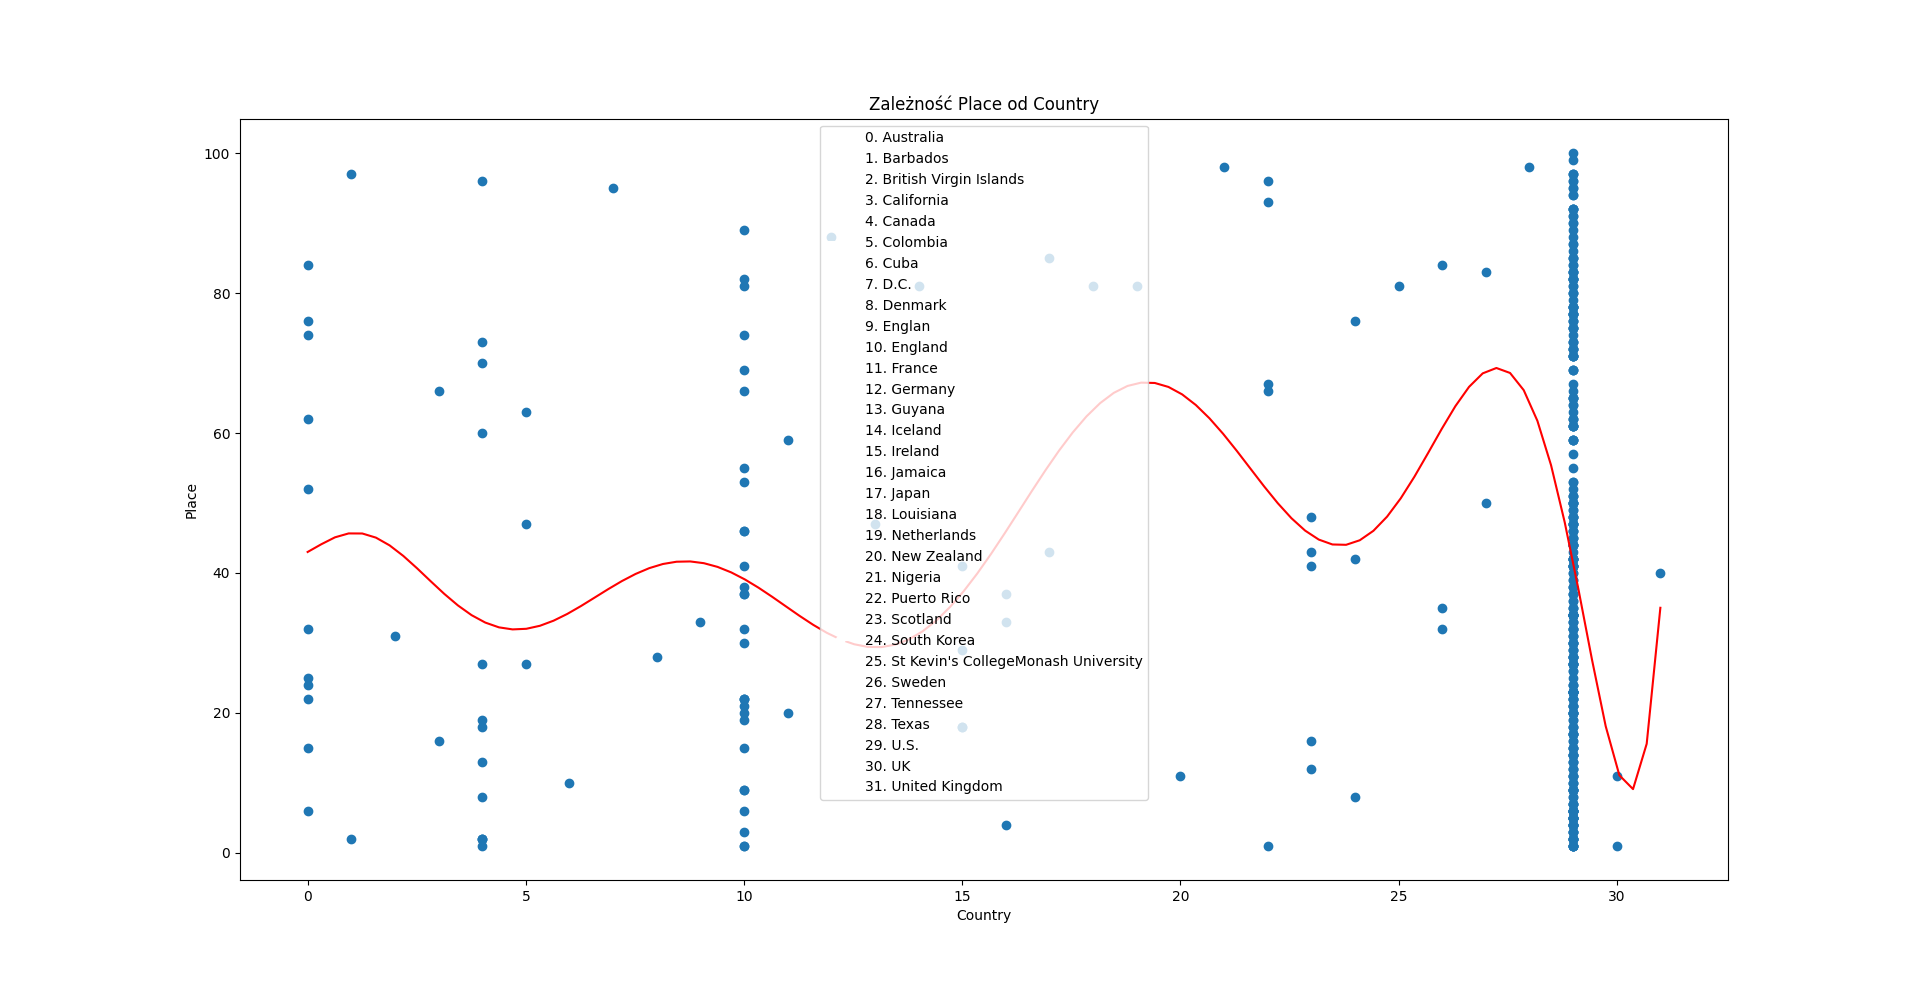
\includegraphics[width=1\textwidth]{place_country_graph}  
    \caption{Przybliżenie wielomianem zależności miejsca w rankingu od kraju pochodzenia}
\end{figure}

\begin{figure}[h]
    \centering
    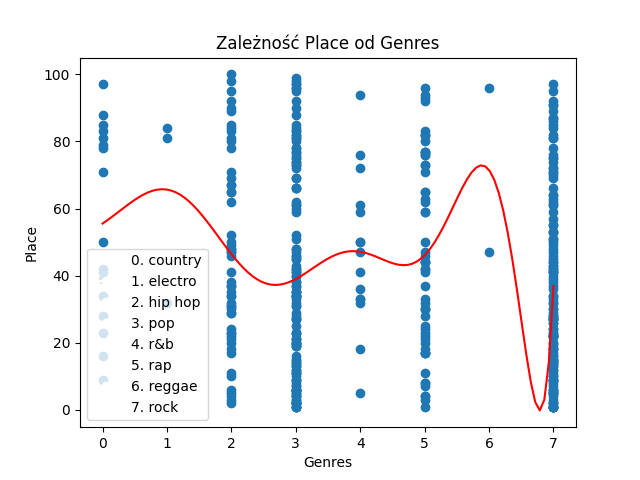
\includegraphics[width=1\textwidth]{place_genres_graph}  
    \caption{Przybliżenie wielomianem zależności miejsca w rankingu od gatunków muzycznych}
\end{figure}

\begin{figure}[h]
    \centering
    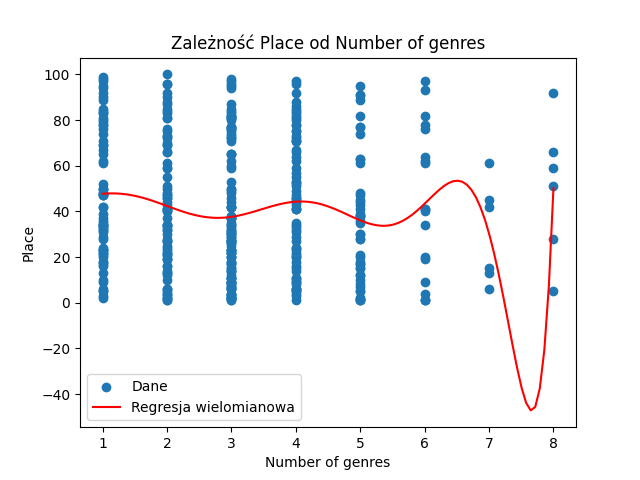
\includegraphics[width=1\textwidth]{place_number_of_genres_graph}  
    \caption{Przybliżenie wielomianem zależności miejsca w rankingu od różnorodności artysty}
\end{figure}

\begin{figure}[h]
    \centering
    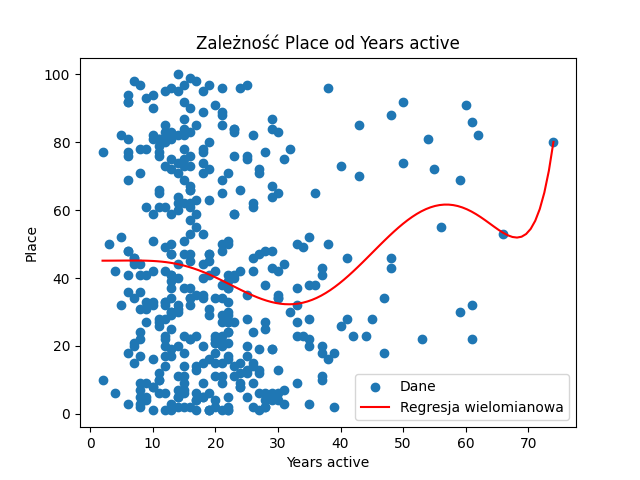
\includegraphics[width=1\textwidth]{place_years_active_graph}  
    \caption{Przybliżenie wielomianem zależności miejsca w rankingu od lat aktywności}
\end{figure}

\subsection{Wnioski}

Dane na jakich operowałem okazały się mało zróżnicowane. Bardzo łatwo wyróżnić cechy artysty, które najczęściej gwarantują czołówkę listy. Ciężko przedstawić przybliżenie wielomianowe w wykresie 7D, dlatego wykresy na pojedynczych cechach przysunęły następujące wnioski:

\begin{itemize}
    \item Największy wpływ na miejsce w rankingu mają wiek oraz lata aktywności artysty, które są ze sobą ściśle powiiązane.
    \item Wiek, który przybliża artystę do pierwszego miejsca najbardziej to około 50 lat.
    \item Lata aktywności, które przybliżają artystę do pierwszego miejsca najbardziej to około 32 lata
    \item Kraj pochodznie artysty nie wpływa znacząco na miejsce na liście. Wynika to z faktu, że przemysł muzyczny zdominowany jest przez wykonwaców ze Stanów Zjednoczonych, którzy mają miejsca w czołówce, jak i w ogonie listy.
    \item Kraj pochodzenia, który najbardziej zbliża artystę do pierwszego miejsca to Stany Zjednoczone. Na drugim miejscu Anglia.
    \item Gatunek muzyczny także nie wpływa znacząco na miejsce na liście. Wynika to z faktu, że wykonwacy sięgający po najbardziej popularne gatunki mają miejsca w rankingu w czołówce, jak i w ogonie.
    \item Gatunek muzyczny najbardziej zbliżający artystę do pierwszego miejsca to rock.
    \item Różnorodność artysty wpływa na miejsce w rankingu bardzo mocno. jest to trzecia cecha, zaraz po wieku i latach aktywności, mająca duże znaczenie.
    \item Liczba różnych gatunków muzycznych, po jakie sięga artysta w swojej dyskografii przybliżająca go do pierwszego miejsca na liście to 7 lub 8. Wynika to z faktu, że niewielu wykonawców miesza ze tak dużo gatunków. Stąd posiadamy mało danych na ich temat, a przeważnie zajmują wysokie miejsce na liście.
    \item Płeć wpływa na miejsce artystyw rankingu nieznacząco. 
    \item Artystów płci męskiej jest o wiele więcej, jednak to kobiety zajmują wyższe miejsca na liście. 
\end{itemize}

\end{document}
